%%%%%%%%%%%%%%%%%%%%%%%%%%%%%%%%%%%%%%%%%%%%%%%%%%%%%%%%%%
\section{Overview of the Proposed Approach}
\label{sect:overviewApproach}
%%%%%%%%%%%%%%%%%%%%%%%%%%%%%%%%%%%%%%%%%%%%%%%%%%%%%%%%%%

This section presents our basic idea of incorporating behavior aspects into a domain model in order to increase its expressiveness. Within our method, structural and behavioral aspects are represented by a so-called unified model and an activity graph, respectively. They are then combined for a whole domain model.

%%%%%%%%%%%%%%%%%%%%%%%%%%%%%%%%%%%%%%%%%%%%%%
\subsection{Basic Idea}
%%%%%%%%%%%%%%%%%%%%%%%%%%%%%%%%%%%%%%%%%%%%%%

\begin{figure}[ht]
\begin{center}
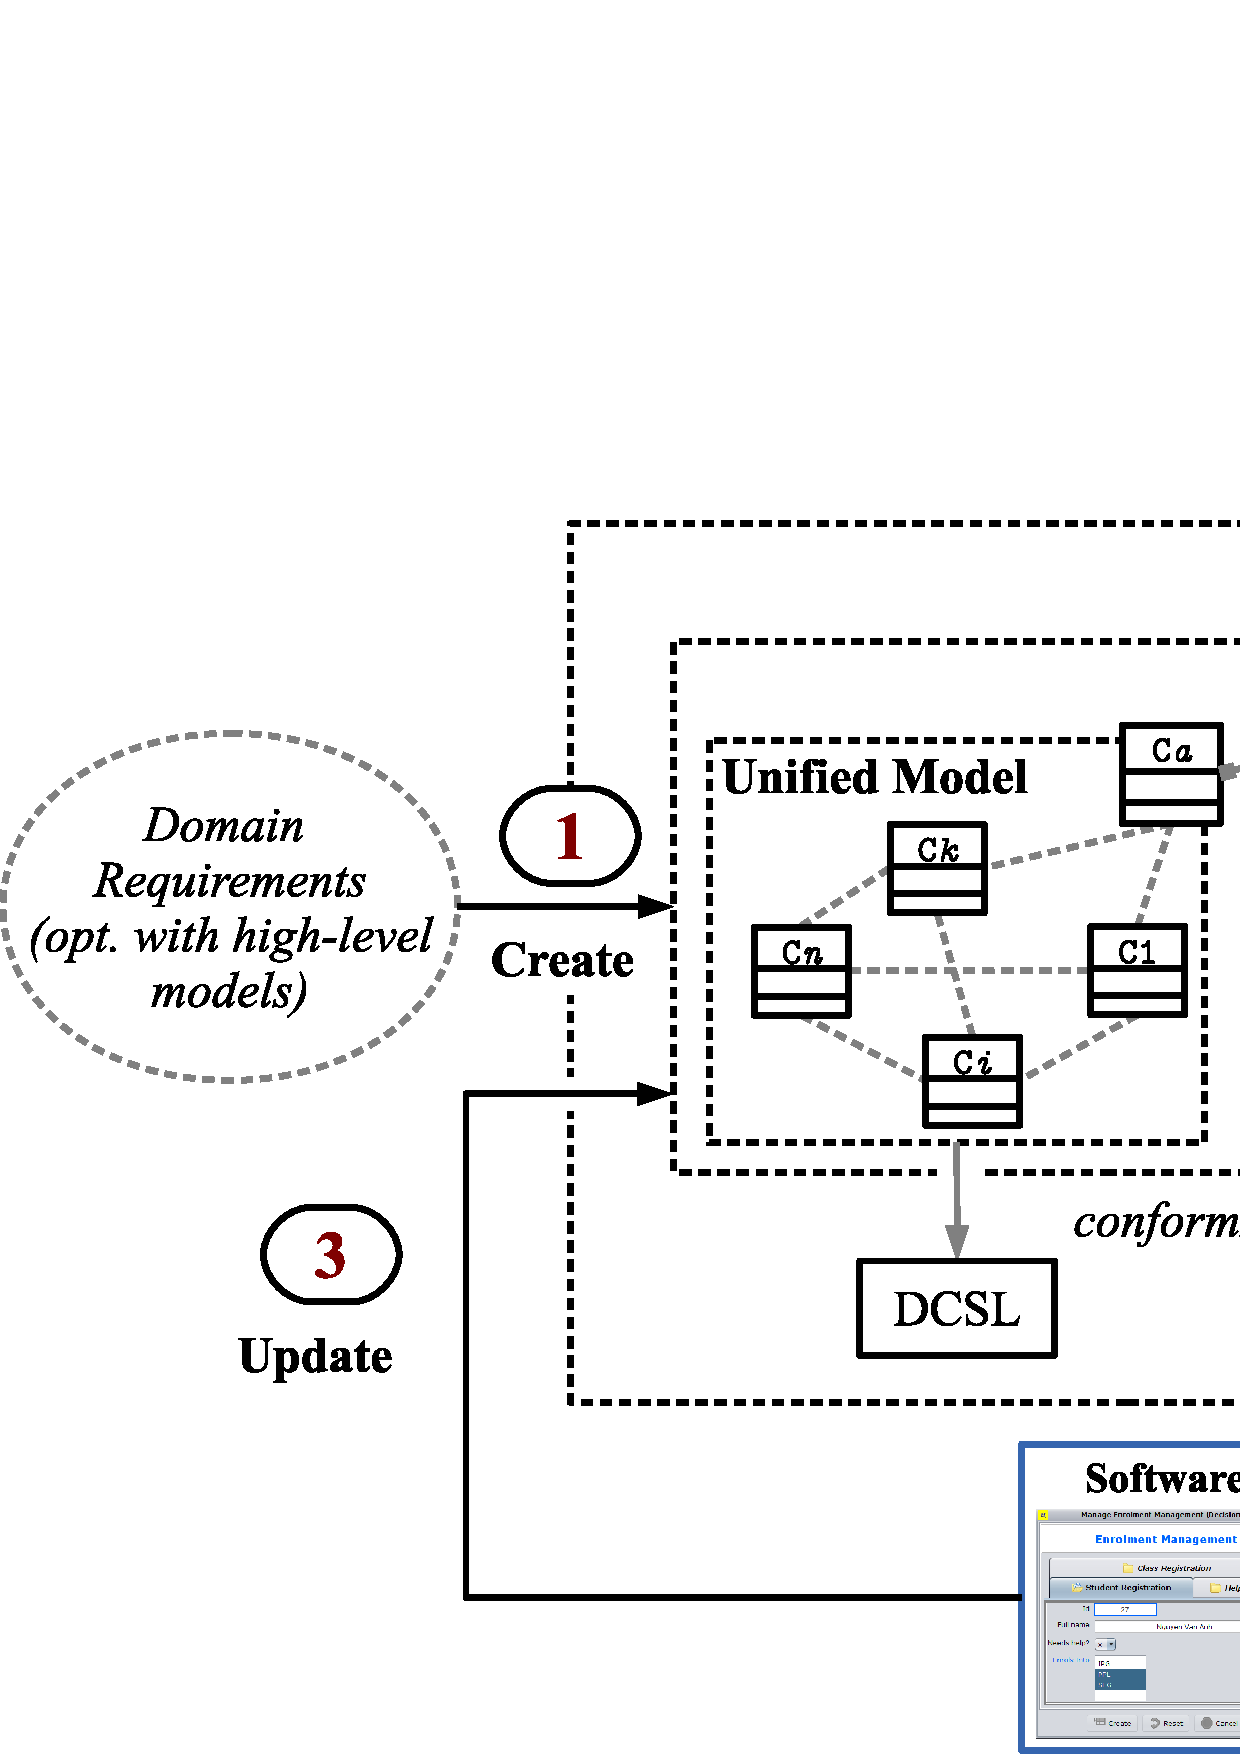
\includegraphics[scale=0.37 %0.26
  ]{method-overview}
\end{center}
\caption{An overview of our method.} %
\label{fig:method-overview}
\end{figure}

%Modeling a software system in DDD requires a domain model to represent both structural and behavioral aspects of the system.
%
%Within our method, we express these using a combination of \textbf{unified domain model} and \textbf{activity graph}.
%
Figure~\ref{fig:method-overview} shows our proposed method.
%, which has been refined from the method that we introduced in~\cite{le_domain_2018}. 
The figure highlights a unified model and its combination with an activity graph. Here, we consider the unified model as an extended domain model in MOSA~\cite{le_domain_2018}. This model, which is expressed in \dcsl, extends the conventional DDD's domain model~\cite{evans_domain-driven_2004} with the domain-specific features of UML activity diagram. Among the essential features that are supported include activity class (\eg class \clazz{C_a} in Figure~\ref{fig:method-overview}), which represents an activity. We use the activity class of each unified model as a pivot with which to define the activity graph. Each activity class is attached to an activity graph that describes the behavioral logic of the represented activity. The activity graphs are expressed in the language \agl~that will be explained in Section~\ref{sect:agl}.

Hence, conceptually our method consists in iteratively performing three steps. The first step takes as input the domain requirements, optionally expressed in some high-level models (\eg, UML class and activity diagrams), and creates a set of initial unified models and associated activity graphs. At this stage, the models and their graphs may be incomplete and, thus, need to be refined in subsequent iterations. The second step takes as input the unified models and graphs and uses MOSA to automatically generate a GUI- and module-based software. This software is presented to the domain expert to get feedbacks. If there are feedbacks, then the third step updates the unified models and graphs and the cycle continues. If, on the other hand, the domain expert is satisfied with the models and graphs, then the cycle ends.

%%%%%%%%%%%%%%%%%%%%%%%%%%%%%%%%%%%%%%%%%%%%%%%%%%%%%%%%%%
\subsection{Unified Model}
%%%%%%%%%%%%%%%%%%%%%%%%%%%%%%%%%%%%%%%%%%%%%%%%%%%%%%%%%%

In principle, unified model is a \dcsl~model that realizes what we term the UML \textit{unified class model}. This model extends the conventional domain model~\cite{evans_domain-driven_2004} with a domain-specific structure from the activity modeling domain.
%
\begin{definition} \label{def:unified-class-model}
	A \textbf{unified class model} is a domain model extended with the following features:
	
	\begin{itemize}%[leftmargin=*]
		\item \textbf{activity class}: a domain class that represents the activity.
		\item \textbf{data component class} (or \textbf{data class} for short): a domain class that represents each data store.
		\item \textbf{control component class} (or \textbf{control class}): captures the domain-specific state of a control node. A control class that represents (does not represent) a control node is named after (resp. the negation of) the node type; \eg, decision (non-decision) class, join (non-join) class, \etc
		\item \textbf{activity-specific association}: an association between each of the following class pairs:
		\begin{itemize}
			\item activity class and a merge class.
			\item activity class and a fork class.
			\item a merge (resp. fork) class and a data class that represents the data store of an action node connected to the merge (resp. fork) node.
			\item activity class and a data class that does not represent the data store of an action node connected to either a merge or fork node.
		\end{itemize}        	
	\end{itemize}
	%
	We will collectively refer to the data and control classes of an activity class model as \textbf{component classes}. \qed
\end{definition}

Note that the representation scheme in the above definition does not cover \textit{all} the possible associations among the component classes. It focuses only on the activity-specific ones. 
%Other domain-specific associations may be introduced if needed.
%
These associations play two important roles. First, they explicitly model the links between domain-specific states of the activity nodes. Second, they are used to incorporate the modules of the data and control classes into the containment tree of the activity module, thereby promoting this module as the main module for managing the entire activity.

The condition imposed on the fourth class pair of activity-specific association stems from the fact that there is no need to explicitly define the association between an activity class and a data class that represents the data store of an action node connected to either a merge or fork node. Such a data class is `indirectly' associated to the activity class, via two associations: one is between it and the merge or fork class (the third class pair), and the other is between the activity class and this control class (the first or second class pair).

%\subsection{Activity Domain Model}
\begin{definition} \label{def:unified-model}
	A \textbf{unified model} is a \dcsl~model that realizes an unified class model as follows:
	\begin{itemize}%[leftmargin=*]
		\item a domain class $ c_a $ (called the \textbf{activity domain class}) to realize the activity class.
		\item the domain classes $ c_1,\dots,c_n $ to realise the component classes.
		\item let $ c_{i_1},\dots,c_{i_k} \in \{c_1,\dots,c_n\} $ realize the non-decision and non-join component classes, then $ c_a,c_{i_1},\dots,c_{i_k} $ contain associative fields that realize the corresponding association ends of the relevant activity-specific associations. \qed
	\end{itemize}
\end{definition}

In the remainder of this paper, to ease notation we will use \textbf{activity class} to refer to the activity domain class $ c_a $ and \textbf{component class} to refer to the $ c_1,\dots,c_n $. 
%We will further assume the existence of a boolean function named \func{activityClass}{:} \clazz{Class} $\rightarrow$ \clazz{Boolean}, which returns \code{true} or \code{false} depending on whether or not a domain class is an activity class.
%
\subsection*{Example: Unified model}
%
\begin{figure*}[ht]
	\begin{center}
		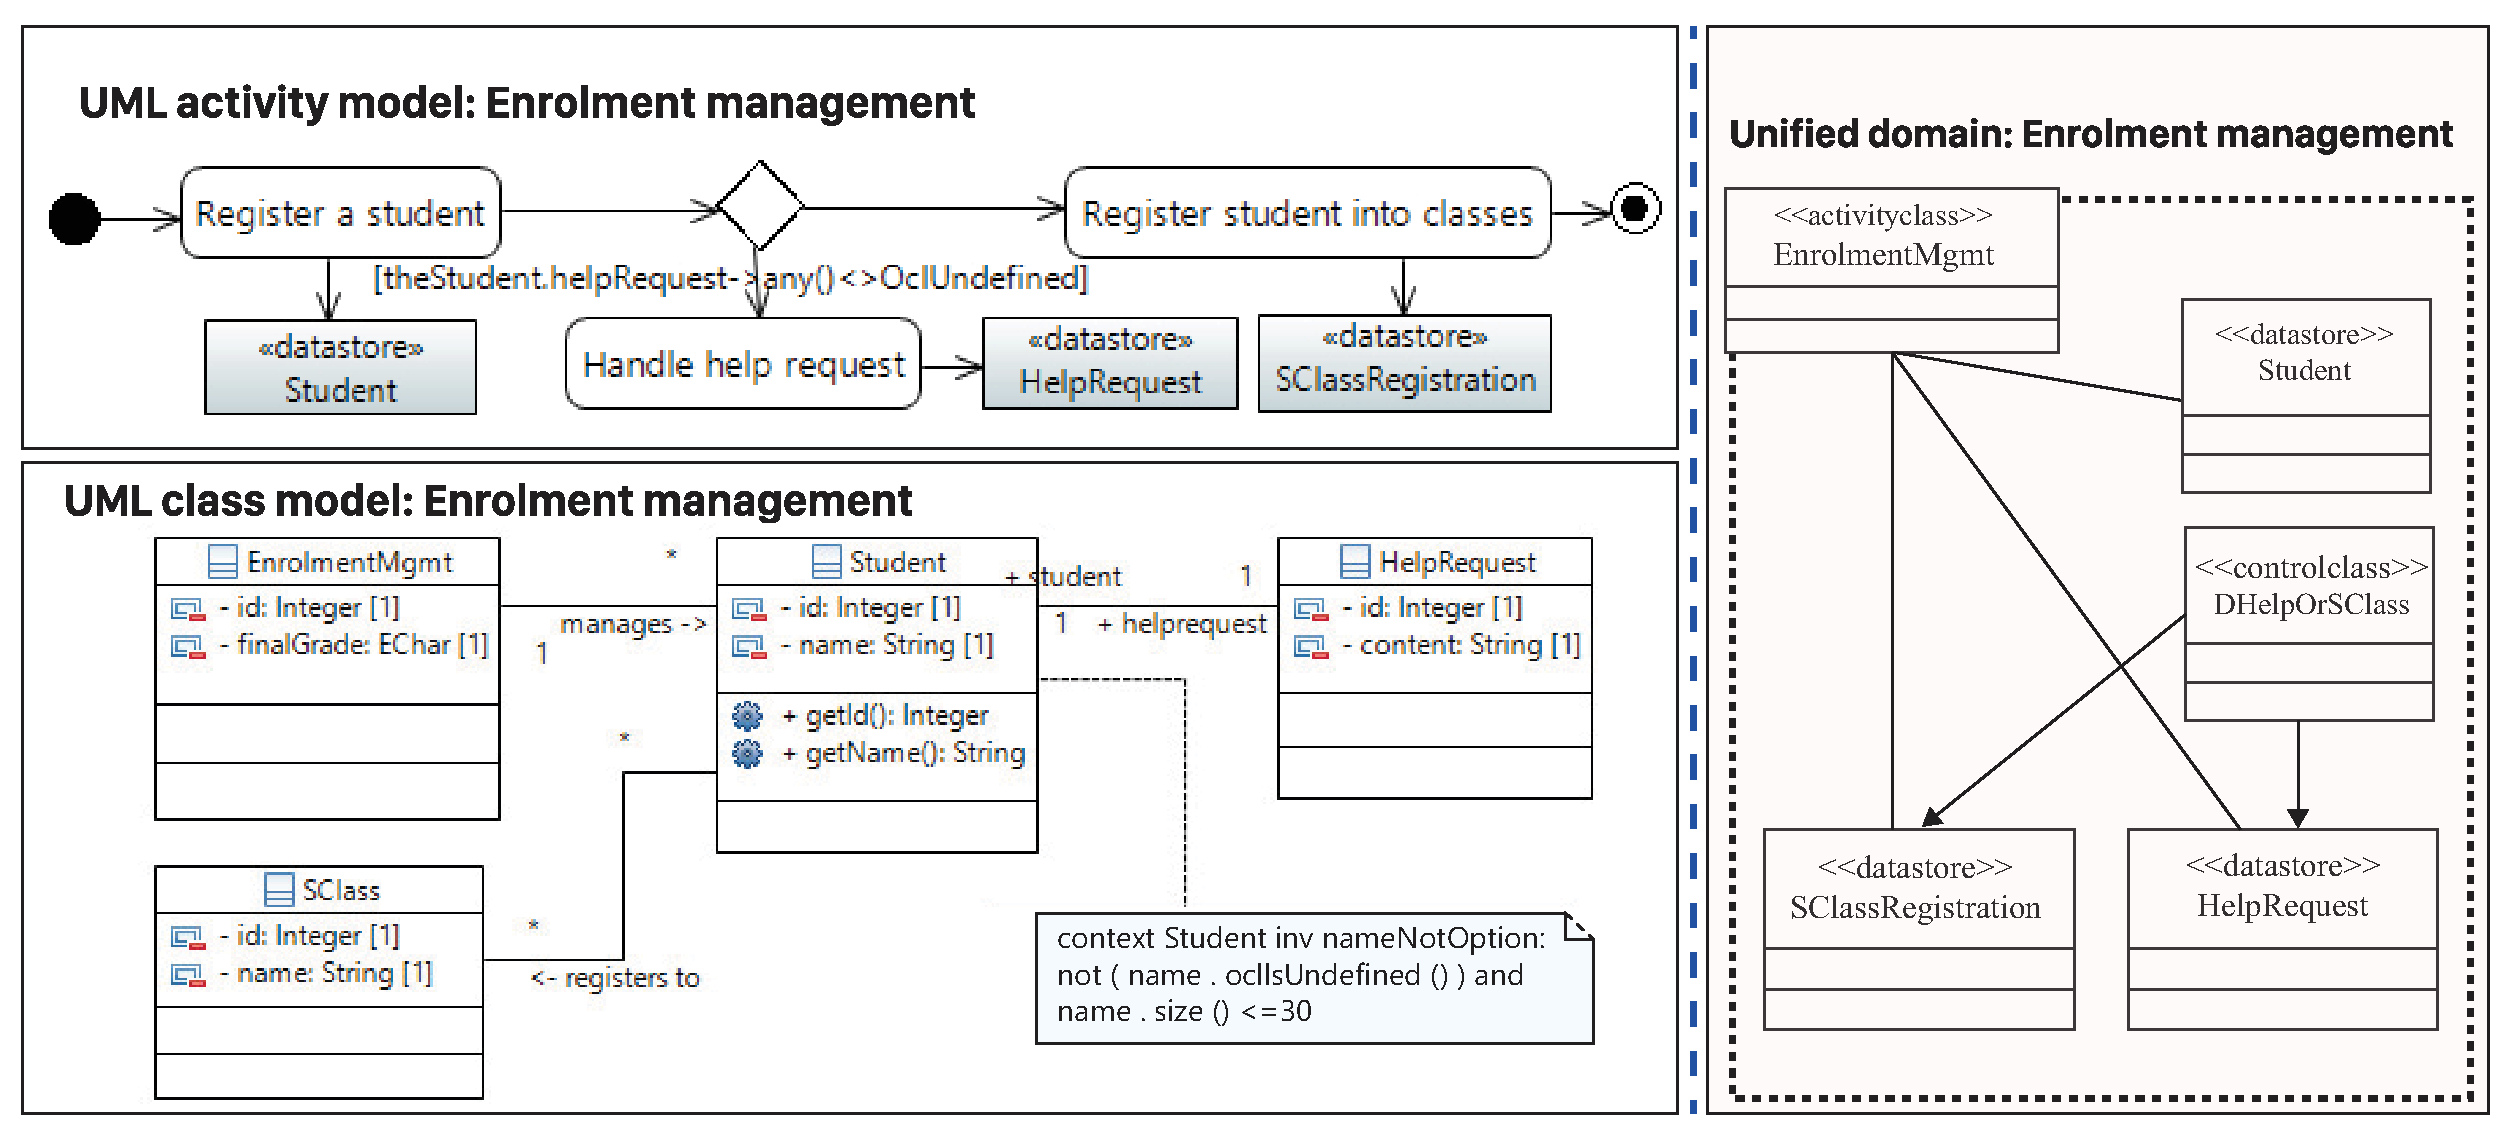
\includegraphics[scale=0.28]{unified-model-example}
	\end{center}
	\caption{(A: Left) The UML activity and class models of a \courseman~software variant that handles the enrollment management activity; (B: Right) The unified model that results.} %
	\label{fig:unified-model-example}
\end{figure*} 

To illustrate, Figure~\ref{fig:unified-model-example}(A) shows the UML activity and class models of a \courseman~variant that handles the enrollment management activity. In this variant, students are allowed to request help after the initial registration. The accompanied class model is extracted from the \courseman's conceptual model shown in Figure~\ref{fig:arch-model-courseman}.
%
Figure~\ref{fig:unified-model-example}(B) shows the resulted unified model of the activity.
This model consists of five domain classes and realizations of five activity-specific associations. To ease reading, we omit the domain-specific associations that are shown in the UML class model in Figure~\ref{fig:unified-model-example}(A). Class \clazz{EnrolmentMgmt} is the activity class. Class \clazz{DHelpOrSClass} is a decision class, which captures the domain-specific decision logic. The remaining three classes are data classes that realize the three data stores. These data classes also correspond to three domain classes in the UML class model. 

Among the five associations, three associate \clazz{EnrolmentMgmt} and the data classes. These associations are used to bind the modules of these data classes to the containment tree of \clazz{ModuleEnrolmentMgmt}.
The remaining two associations associate the decision class \clazz{DHelpOrSClass} to two data classes (\clazz{SClassRegistration} and \clazz{HelpRequest}), which realize the data stores connected to the two actions nodes branching of the decision node. These associations are weak dependency associations and only added in this case because the decision logic encapsulated by \clazz{DHelpOrSClass} needs to reference the two data classes.
%
In SubSection~\ref{sect:decisional-pattern}, we will revisit this example in the context of the decisional modeling pattern and present a software GUI that is generated from the model.
